% You should title the file with a .tex extension (hw1.tex, for example)
\documentclass[11pt]{article}

\usepackage{amsmath}
\usepackage{amssymb}
\usepackage{fancyhdr}
\usepackage{graphicx}

\oddsidemargin0cm
\topmargin-2cm         %I recommend adding these three lines to increase the
\textwidth16.5cm   %amount of usable space on the page (and save trees)
\textheight23.5cm  

\newcommand{\question}[2] {\vspace{.25in} \hrule\vspace{0.5em}
\noindent{\bf #1: #2} \vspace{0.5em}
\hrule \vspace{.10in}}
\renewcommand{\part}[1] {\vspace{.10in} {\bf (#1)}}

\newcommand{\myname}{Tanay Gavankar}
\newcommand{\myandrew}{tgavanka@andrew.cmu.edu}
\newcommand{\myhwnum}{Homework 2}

\setlength{\parindent}{0pt}
\setlength{\parskip}{5pt plus 1pt}

\pagestyle{fancyplain}
\lhead{\fancyplain{}{\textbf{HW\myhwnum}}}          % Note the different brackets!
\rhead{\fancyplain{}{\myname\\ \myandrew}}
\chead{\fancyplain{}{10-601}}

\begin{document}

\medskip                            % Skip a "medium" amount of space
                                   % (latex determines what medium is)
                                   % Also try: \bigskip, \littleskip




\thispagestyle{plain}
\begin{center}                      % Center the following lines
{\Large 10-601 Assignment \myhwnum} \\
\myname \\
\myandrew \\
Due: 9/28/12 \\
\end{center}




\question{1.1}{Naive Bayes: Basic Concepts}
\part{a}
Yes, this is the assumption that Naive Bayes makes. 

\part{b}
No. Since all we know that $X$ is independent of $Y|Z$, we do not know if $X$ is independent of $Y$ in general.

\part{c}
$J*(X^n)$. (Note that since this covers the entire space, we'd only have to calculate $J*(X^n)-1$ of them, as the remaining one would be $1-\sum{P(X_i|Y)}$.)

\part{d}
There are $n$ distinct $\mu_{ij},\sigma_{ij}$ because there is one for each $x_i$.

\part{e}
When estimating $Y$, the denominator does not depend on what we are trying to calculator the probability for, so the denominator is effectively constant. 

\part{f}
Yes, we can calculate P(X) from the parameters estimated by Naive Bayes by using relative frequencies of the training sett.

\question{1.2}{Naive Bayes: Parameter elimination}
\part{a}
$\hat{\theta_{1k}} = \frac{\sum_1^M{x_{1j}}}{M}$

\part{b}
\begin{eqnarray*}
\mu^{mle} &=& arg max_{\mu} P(X_1, X_2, ...X_n | Y)\\
&=& arg max_{\mu} \prod_{i=1}^n{P(X_i|Y)}\\
&=& arg max_{\mu} \sum_{i=1}^n{log(P(X_i|Y))}\\
&=& arg max_{\mu} \sum_{i=1}^n{log(\frac{1}{\sigma \sqrt{2\pi}}exp(\frac{-(X_{i}-\mu_{i})^2}{2\sigma^2}))}\\
&=& arg max_{\mu}\frac{1}{\sigma \sqrt{2\pi}} \sum_{i=1}^n{\frac{-(X_{i}-\mu_{i})^2}{2\sigma^2}}\\
&=& arg min_{\mu}\sum_{i=1}^n{(X_{i}-\mu_{i})^2}\\
\end{eqnarray*}

We want to minimize this, so take the derivative and set to zero, and solve.

\begin{eqnarray*}
0 &=& \frac{\partial}{\partial \mu}\sum_{i=1}^n{(X_{i}-\mu_{i})^2}\\
&=& -\sum_{i=1}^{n}{2(X_{i}-\mu)}\\
\Rightarrow \mu^{mle} &=& \frac{1}{n}\sum_{i=1}^{n}{X_i}\\
\end{eqnarray*}

\question{2}{Regularized Multi-Class Logistic Regression}
\part{a}
Let $l$ be the $lth$ training data entry.
\begin{eqnarray*}
W &\leftarrow& argmax_W \prod_l{P(Y^l=k|X^l,W)/(\frac{\lambda}{2}||W||^2)}\\
l(W) &=& \sum_{l \in D}{lnP(Y^l|X^l,W)} - ln(\frac{\lambda}{2}||W||^2)\\
l(W) &=& \sum_{l \in D}{ln(  \frac{exp(w_k^Tx)}{1+\sum_{t=1}^{K-1}{exp(w_t^Tx)}}  ) - ln(\frac{\lambda}{2}||W||^2)}\\
l(W) &=& \sum_{l \in D}{ln(exp(w_k^Tx)) - ln(1+\sum_{t=1}^{K-1}{exp(w_t^Tx)})) - ln(\lambda) + ln(2) - 2ln(||W||)}\\
l(W) &=& \sum_{l \in D}{w_k^Tx - ln(1+\sum_{t=1}^{K-1}{exp(w_t^Tx)})) - ln(\lambda) + ln(2) - 2ln(||W||)}\\
\end{eqnarray*}

\part{b}
\begin{eqnarray*}
l(W) &=& \sum_{l \in D}{lnP(Y^l|X^l,W)} - ln(\frac{\lambda}{2}||W||^2)\\
\end{eqnarray*}
By adding the penalty term, we have a new objective to maximize. However, maximizing this new objective corresponds to calculating the MAP estimate for W under the assumption that the prior distribution $P(W)$ is a Normal distribution with mean zero, and a variance related to $\frac{1}{\lambda}$. If $P(W)$ is a zero mean Gaussian distribution, then $lnP(W)$ yields a term proportional to $||W||^2$, so we can work with that.
\begin{eqnarray*}
l(W) &=& \sum_{l \in D}{lnP(Y^l|X^l,W)} - lnP(W)\\
\frac{\partial l(W)}{\partial w_i} &=& \sum_l{X_i^l(Y^l-\hat{P}(Y^l=1|X^l,W))-\lambda w_i}\\
&=& \eta\sum_l{X_i^l(Y^l-\hat{P}(Y^l=1|X^l,W))-\eta\lambda w_i}\\
\end{eqnarray*}

\part{c}
\begin{eqnarray*}
w_i \leftarrow w_i + \eta\sum_l{X_i^l(Y^l-\hat{P}(Y^l=1|X^l,W))-\eta\lambda w_i}\\
w_i \leftarrow w_i + v\sum_l{X_i^l(Y^l-\hat{P}(Y^l=1|X^l,W))-v\lambda w_i}\\
\end{eqnarray*}

\part{d}
Yes, it will converge to a global maximum because that is where the MLE appears.

\question{3}{Generative-Discriminative Classifiers}
\part{a}
Since $X_i$ are boolean variables, we can use a single parameter to define $P(X_i|Y=y_k)$. Let $\theta_{i1} =  P(X_i=1|Y=1)$. This means that $P(X_i=0|Y=1)=(1-\theta_{i1})$ and $P(X_i=1|Y=0)=\theta_{i0}$. This all means that $P(X_i|Y=1) = \theta_{i1}^{X_i}(1-\theta_{i1})^{(1-X_i)}$. Also, let $P(Y=1)=\pi$.

\begin{eqnarray*}
P(Y=1|X) &=& \frac{P(Y=1)P(X|Y=1)}{P(Y=1)P(X|Y=1)+P(Y=0)P(X|Y=0)}\\
&=& \frac{1}{1+\frac{P(Y=0)P(X|Y=0)}{P(Y=1)P(X|Y=1)}}\\
&=& \frac{1}{1+exp(ln(\frac{P(Y=0)P(X|Y=0)}{P(Y=1)P(X|Y=1)}))}\\
&=& \frac{1}{1+exp(ln\frac{P(Y=0)}{P(Y=1)} + \sum_i{ln\frac{P(X_i|Y=0)}{P(X_i|Y=1)}})}\\
&=& \frac{1}{1+exp(ln\frac{1-\pi}{\pi} + \sum_i{ln\frac{\theta_{i0}^{X_i}(1-\theta_{i0})^{(1-X_i)})}{\theta_{i1}^{X_i}(1-\theta_{i1})^{(1-X_i)}}})}\\
\end{eqnarray*}

Let's look at only the sum in the denominator.

\begin{eqnarray*}
\sum_i{ln\frac{P(X_i|Y=0)}{P(X_i|Y=1)}} &=&  \sum_i{ln\frac{\theta_{i0}^{X_i}(1-\theta_{i0})^{(1-X_i)}}{\theta_{i1}^{X_i}(1-\theta_{i1})^{(1-X_i)}}}\\
&=& \sum_i{ln(\theta_{i0}^{X_i}(1-\theta_{i0})^{(1-X_i)}) - ln(\theta_{i1}^{X_i}(1-\theta_{i1})^{(1-X_i)})}\\
&=& \sum_i{ln(\theta_{i0}^{X_i}) + ln((1-\theta_{i0})^{(1-X_i)}) - ln(\theta_{i1}^{X_i}) - ln((1-\theta_{i1})^{(1-X_i)})}\\
&=& \sum_i{X_iln(\theta_{i0}) + (1-X_i)ln(1-\theta_{i0}) - X_iln(\theta_{i1}) - (1-X_i)ln(1-\theta_{i1})}\\
&=& \sum_i{X_iln(\theta_{i0}) + ln(1-\theta_{i0}) - X_iln(1-\theta_{i0}) - X_iln(\theta_{i1}) - ln(1-\theta_{i1}) + X_iln(1-\theta_{i1})}\\
\end{eqnarray*}

\part{b}
Assuming all the NB assumptions are satisfied, both NB and LR will have identical results because NB can be mapped to LR. 

\part{c}
Assuming the conditional independence assumption of NB is not satisfied, then the NB bias will cause it to perform less accurately than LR in the limit.

\part{d}
It is not possible for the LR estimated parameters to calculated P(X) because LR calculates P(Y|X), and so since X has to be given, a probability cannot be calculated for it.

\question{4}{Programming}
\part{a}
These results are for the full data set.\\
    \begin{tabular}{|l|l|l|}
        \hline
        Algorithm & Naive Bayes & Logistic Regression \\ \hline
        Learning Time (s) & 16.162 & 88.745 \\ \hline
        Training Classification Time (s) & 28.41 & 12.012 \\ \hline
        Training Classification Accuracy (\%) & 96.93 & 98.23 \\ \hline
        Test Classification Time (s) & 11.255 & 4.763 \\ \hline
        Test Classification Accuracy (\%) & 98.23 & 97.79 \\
        \hline
    \end{tabular}

As you can see, both methods were pretty accurate given the large training data set size.

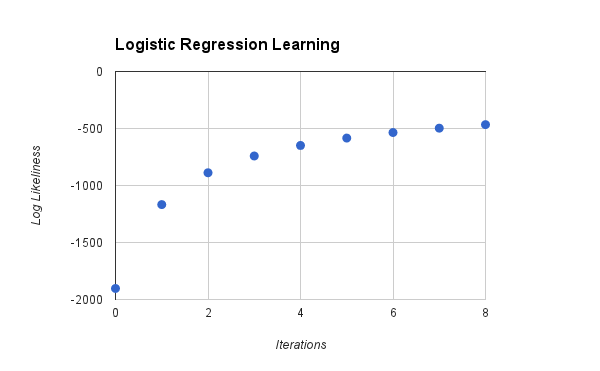
\includegraphics[scale=0.75]{4a.png}\\

\part{b}
These results are for the 1000 best feature-selected data set.\\

    \begin{tabular}{|l|l|l|}
        \hline
        Algorithm                             & Naive Bayes & Logistic Regression \\ \hline
        Learning Time (s)                     & 3.189       & 21.470              \\ 
        Training Classification Time (s)      & 5.507       & 2.342               \\ 
        Training Classification Accuracy (\%) & 95.89       & 97.79               \\ 
        Test Classification Time (s)          & 2.176       & 0.929               \\ 
        Test Classification Accuracy (\%)     & 97.90       & 97.23               \\
        \hline
    \end{tabular}

As you can see, the feature-selected data sets were significantly faster while maintaining comparable accuracy. While the accuracy of the feature-selected data was slightly lower on all accounts, the largest difference was with NB training accuracy, decreasing by 1.04\% between the full and feature-selected data sets. 

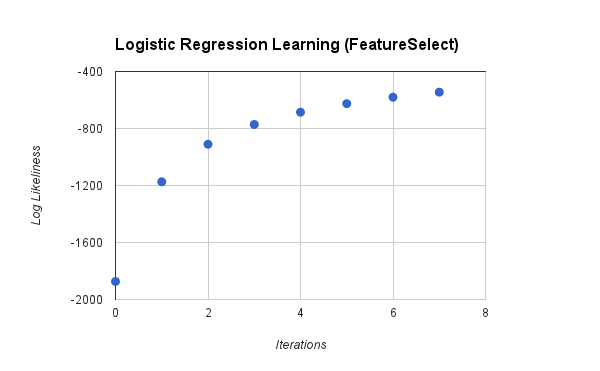
\includegraphics[scale=0.75]{4b.png}\\

\part{c}

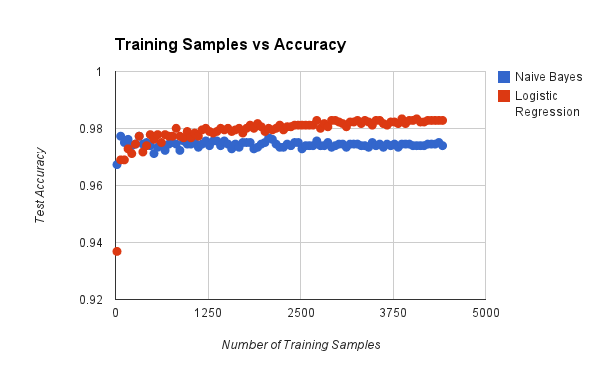
\includegraphics[scale=0.75]{4c.png}\\
This plot shows that the limit for logistic regression has a higher accuracy than Naive Bayes. This means that the Naive Bayes assumptions do not hold completely in this data set. The Naive Bayes assumptions, if they held, would imply that the limit for accuracy would be equal for the two algorithms. However, because there is more noise/variance (lower accuracy) in Naive Bayes, this means that its assumptions are not completely valid.

\end{document}
